%=======================================================
%	PACKAGES AND THEMES
%=======================================================
\documentclass[8pt]{beamer}
\mode<presentation> {
\usepackage{etex}
\usetheme{Boadilla}
\definecolor{navyblue}{rgb}{0.0, 0.0, 0.5}
\definecolor{dkgreen}{rgb}{0,0.6,0}
\definecolor{gray}{RGB}{64, 64, 64}
\definecolor{teal}{RGB}{0, 102, 102}
\definecolor{mauve}{rgb}{0.58,0,0.82}
\usecolortheme[named = navyblue]{structure}
\setbeamercolor{normal text}{fg = gray}
\setbeamercolor{frametitle}{fg = white, bg = navyblue}
\setbeamerfont{framesubtitle}{size = \normalsize}
\setbeamerfont{caption}{size=\footnotesize}
\setbeamercolor{page number in head/foot}{fg = gray}
\setbeamertemplate{footline}%[frame number]
}


\usepackage{graphicx} % Allows including images
\usepackage{booktabs} % Allows the use of \toprule, \midrule and \bottomrule in tables
\usepackage{multicol}
\usepackage[export]{adjustbox}
\usepackage{colortbl}
\usepackage{graphicx} 

\usepackage{tikz}
\usepackage{fancybox}
\usepackage[absolute, overlay]{textpos}
\usepackage{multirow}
\usepackage{siunitx}
\usepackage{tcolorbox}


\usepackage{tikz}
\usepackage{calc}
\newlength{\outerradius}
\newlength{\innerradius}
\setlength{\outerradius}{0.50cm}
\setlength{\innerradius}{0.35cm}

%Damit wir Quellcode nutzen können.
\usepackage{listings}
\lstset{numbers=left,
	numberstyle=\tiny,
	numbersep=5pt,
	breaklines=true,
	showstringspaces=false,
	frame=l ,
	xleftmargin=15pt,
	xrightmargin=15pt,
	basicstyle=\ttfamily\scriptsize,
	stepnumber=1,
	keywordstyle=\color{blue},          % keyword style
  	commentstyle=\color{dkgreen},       % comment style
  	stringstyle=\color{mauve}         % string literal style
}
%Sprache Festelegen
\lstset{language=R}


%=======================================================
%	TITLE PAGE
%=======================================================

\title{\textbf{Descriptive Network Analysis A}\\
	      {\color{teal}{--Seminar--}}}

\author{Yasemin Aslan)}

\institute
{
SPRU (Science Policy Research Unit) \\
Business School\\
University of Sussex \\

\medskip

\medskip

\medskip

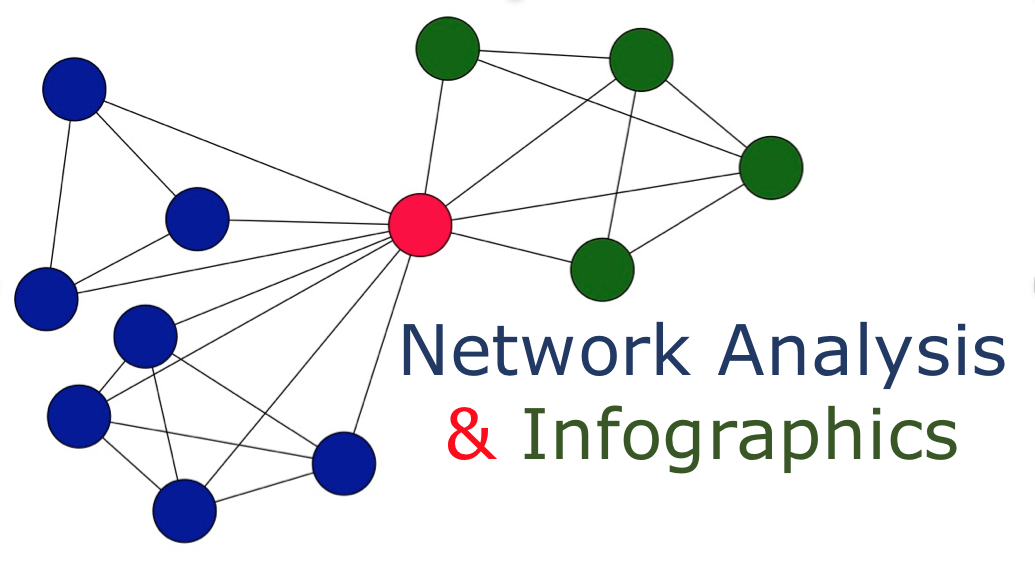
\includegraphics[width=2.5cm]{../_shared_pics/logo}

\medskip

\textit{{\color{dkgreen}{Week 4: 18 February 2022}}}\\
}


\date{} % Date, can be changed to a custom date

\begin{document}

\begin{frame}
\titlepage % Print the title page as the first slide

\begin{textblock*}{10pt}(0pt, 0.9\textheight)

\includegraphics[width=4cm]{../_shared_pics/SPRU.png}
\end{textblock*}

\end{frame}



%=======================================================
%	Learning outcomes
%=======================================================


\begin{frame}
\frametitle{\insertsection}
\framesubtitle{Learning Outcomes}

\centering
\begin{tabular}{lp{5.5cm}l}
\toprule
\multicolumn{2}{l}{\textbf{Learning outcome}} & \textbf{Assessment mode}\\
\hline
\\
1 & 
Explain the concept of network and list the main network indicators & 
ESS\\
\\
2 &  
Describe and apply the major techniques for the collection of network data and their statistical analysis & 
ESS, GPN + GWS\\
\\
\rowcolor{green!20}3 & 
Identify the main characteristics of networks by means of network measures  & 
ESS, GPN + GWS\\
\\
4 &
Employ network analysis techniques to produce network data-based infographics & 
GPN + GWS\\
\\
\bottomrule
\multicolumn{3}{l}{\scriptsize Note: ESS: Essay; GPN: Group Presentation; GWS: Group Written Submission}\\
\end{tabular}

\end{frame}

%------------------------------------------------


%=======================================================
%	Intro slides
%=======================================================

\begin{frame}
\frametitle{Overview}
\tableofcontents[hideallsubsections]
\end{frame}

%------------------------------------------------






%=======================================================
% Network-level measures [recap]
%=======================================================
\section{Network-level measures [recap]}
%------------------------------------------------

\bgroup
\setbeamercolor{background canvas}{bg = navyblue}
\begin{frame}[plain]{}
\begin{center}
\color{white}{\Huge\insertsection}
\end{center}
\end{frame}
\egroup

%------------------------------------------------

\begin{frame}
\frametitle{\insertsection}
\framesubtitle{Interpretation}

\footnotesize
\centering
\begin{tabular}{lp{7.5cm}}
\toprule
\textbf{Measure} & \textbf{Interpretation}\\
\hline
Diameter                        & Maximum time/resources for communication, transfer, ...\\
\\
APL                             & Average time/resources for communication, transfer, ...\\
\\
Density                         & Connectivity of a network \\
\\
Components                      & Presence of unconnected groups, bridging opportunities, ... \\
\\
Cutpoints and bridges           & Vulnerability/resilience of a network\\
\\
Point/Line connectivity         & Vulnerability/resilience of a network\\
\\
Cliques                         & Highly connected sub-groups, exclusion, ...\\
\\
Inclusiveness                   & Presence of unconnected nodes, exclusion, ... \\    
\\
Reachable pairs                 & Unconnected nodes or groups, bridging opportunities, ... \\
\\
Transitivity                    & Social interactions, `friends of my friends are my friends', ... \\

\bottomrule
\end{tabular}

\end{frame}

%------------------------------------------------



%=======================================================
% Network-level measures in igraph
%=======================================================
\section{Network-level measures in \textit{igraph}}
%------------------------------------------------

\bgroup
\setbeamercolor{background canvas}{bg = navyblue}
\begin{frame}[plain]{}
\begin{center}
\color{white}{\Huge\insertsection}
\end{center}
\end{frame}
\egroup

%------------------------------------------------

\begin{frame}
\frametitle{\insertsection}

Your source of all igraph functions: \url{http://igraph.org/r/doc/}

\end{frame}

%------------------------------------------------


\begin{frame}
\frametitle{\insertsection}

\footnotesize
\centering
\begin{tabular}{lp{7.5cm}}
\toprule
\textbf{Measure} & \textbf{igraph function}\\
\hline
Diameter                        & \textbf{diameter(...)}\\
\\
APL                             & \textbf{mean\_distance(...)}\\
\\
Density                         & \textbf{edge\_density(...)}\\
\\
Components                      & \textbf{components(...)}\\
\\
Cutpoints and bridges           & \textbf{articulation\_points(...)} [no function to identify bridges]\\
\\
Point/Line connectivity         & \textbf{min\_cut(...)} [no function for line connectivity]\\
\\
Cliques                         & \textbf{cliques(...)} and \textbf{count\_max\_cliques(...)} \\
\\
Inclusiveness                   & [combination of functions] \\    
\\
Reachable pairs                 & [combination of functions] \\
\\
Transitivity                    & \textbf{transitivity(...)} \\

\bottomrule
\end{tabular}

\end{frame}



%%=======================================================
%	Next time ...
%%=======================================================
\section*{Next time ...}
%------------------------------------------------

\bgroup
\setbeamercolor{background canvas}{bg = navyblue}
\begin{frame}[plain]{}
\begin{center}
\color{white}{\Huge\insertsection}
\end{center}
\end{frame}
\egroup

%------------------------------------------------

\begin{frame}
\frametitle{\insertsection}

\begin{itemize}

\item 	\textbf{Lecture: Descriptive network analysis B}
	\begin{itemize}
	\item Node-level measures (centrality measures)
	\end{itemize}
	
		

\medskip
\medskip


\item 	\textbf{Seminar: Descriptive network analysis B}
	\begin{itemize}
	\item Assessment of node-level measures (centrality measures)
	\end{itemize}
	

		
\end{itemize}

\end{frame}

%------------------------------------------------






\end{document}